\chapter{光的颜色与光谱}\label{ch:g8:colors-spectra}

颜色住在哪里？常识说，就在苹果上——
红色正在果皮上。可是把这只苹果搬进
灯光偏深蓝的体育馆，“红”苹果便黑得像煤块。
颜色原来是光、物体与眼睛之间的三方对话，
而这场对话的开场，就是光学中最奇怪的事实：
白光并不是白的。

\section{白光的分解}

\begin{proposition}[白光是一种混合光]\label{prop:g8:colors-spectra:mixture}
普通的“白”光——阳光、灯光——是
多种颜色同时混合而成的。让它穿过一块玻璃棱镜，
混合光便被分开：每种颜色穿过玻璃时偏折的
角度略有不同，于是颜色散开，
形成一条连续的色带，从红色（偏折最小）到紫色（偏折最大）。
这条色带称为\emph{光谱}\index{光谱}，
分开的过程则称为\emph{色散}\index{色散}。
\end{proposition}

\begin{omfigure}
\begin{tikzpicture}[scale=0.85]
  \draw[-Stealth, very thick] (0.2,1.6) -- (3.2,1.6);
  \node[above, font=\small] at (1.5,1.75) {白光};
  \draw[thick, fill=blue!6] (3.4,0.4) -- (4.6,2.8) -- (5.8,0.4)
    -- cycle;
  \draw[red, very thick] (4.85,1.45) -- (9.6,1.15);
  \draw[orange, very thick] (4.85,1.45) -- (9.6,0.85);
  \draw[yellow!75!black, very thick] (4.85,1.45) -- (9.6,0.55);
  \draw[green!65!black, very thick] (4.85,1.45) -- (9.6,0.25);
  \draw[blue, very thick] (4.85,1.45) -- (9.6,-0.05);
  \draw[violet, very thick] (4.85,1.45) -- (9.6,-0.35);
  \node[right, font=\small] at (9.7,1.15) {红色：偏折最小};
  \node[right, font=\small] at (9.7,-0.35) {紫色：偏折最大};
  \node[below, font=\small] at (4.6,0.2) {棱镜};
\end{tikzpicture}

{\small 色散：棱镜使白光这一混合中的每种颜色各按其量偏折，
混合光于是现出原形——
一条从红到紫的光谱。}
\end{omfigure}

\begin{example}[不借助实验室的光谱]\label{ex:g8:colors-spectra:everyday}
大自然和家里的杂物抽屉里到处都是棱镜。彩虹便是这样：
每一滴雨滴都是一个微型的棱镜兼镜子，满天的彩弧
是阳光被无数雨滴色散的结果——总出现在
与太阳\emph{相对}的那半边天空，
这正是彩虹猎人总让太阳在身后的缘故。花园水管喷出的细雾
也能随手造出一道彩虹。CD 的刻纹面
会在天花板上投下小小的光谱；镜子的斜切边
在晴朗的午后会在墙上划出条纹。白光
每当遇到精细结构或倾斜的玻璃时，
它的混合本性便暴露无遗。
\end{example}

\begin{example}[把混合光重新装回去]\label{ex:g8:colors-spectra:newtondisc}
分解的过程也可以反过来。把一个圆盘涂成彩虹色的扇形，
高速旋转，眼睛跟不上转动，
每个位置几乎同时接收到所有颜色——于是读出
的是混合：一种浅淡的灰白色。伟大的物理学家
最先用棱镜分解了阳光，他就曾用这样的圆盘
来论证颜色的合成——他最大胆的一步是
再用一块棱镜接住光谱，把它重新叠合成
一束白色光束：混合性质由此得到双向证明。
\end{example}

\begin{omfigure}
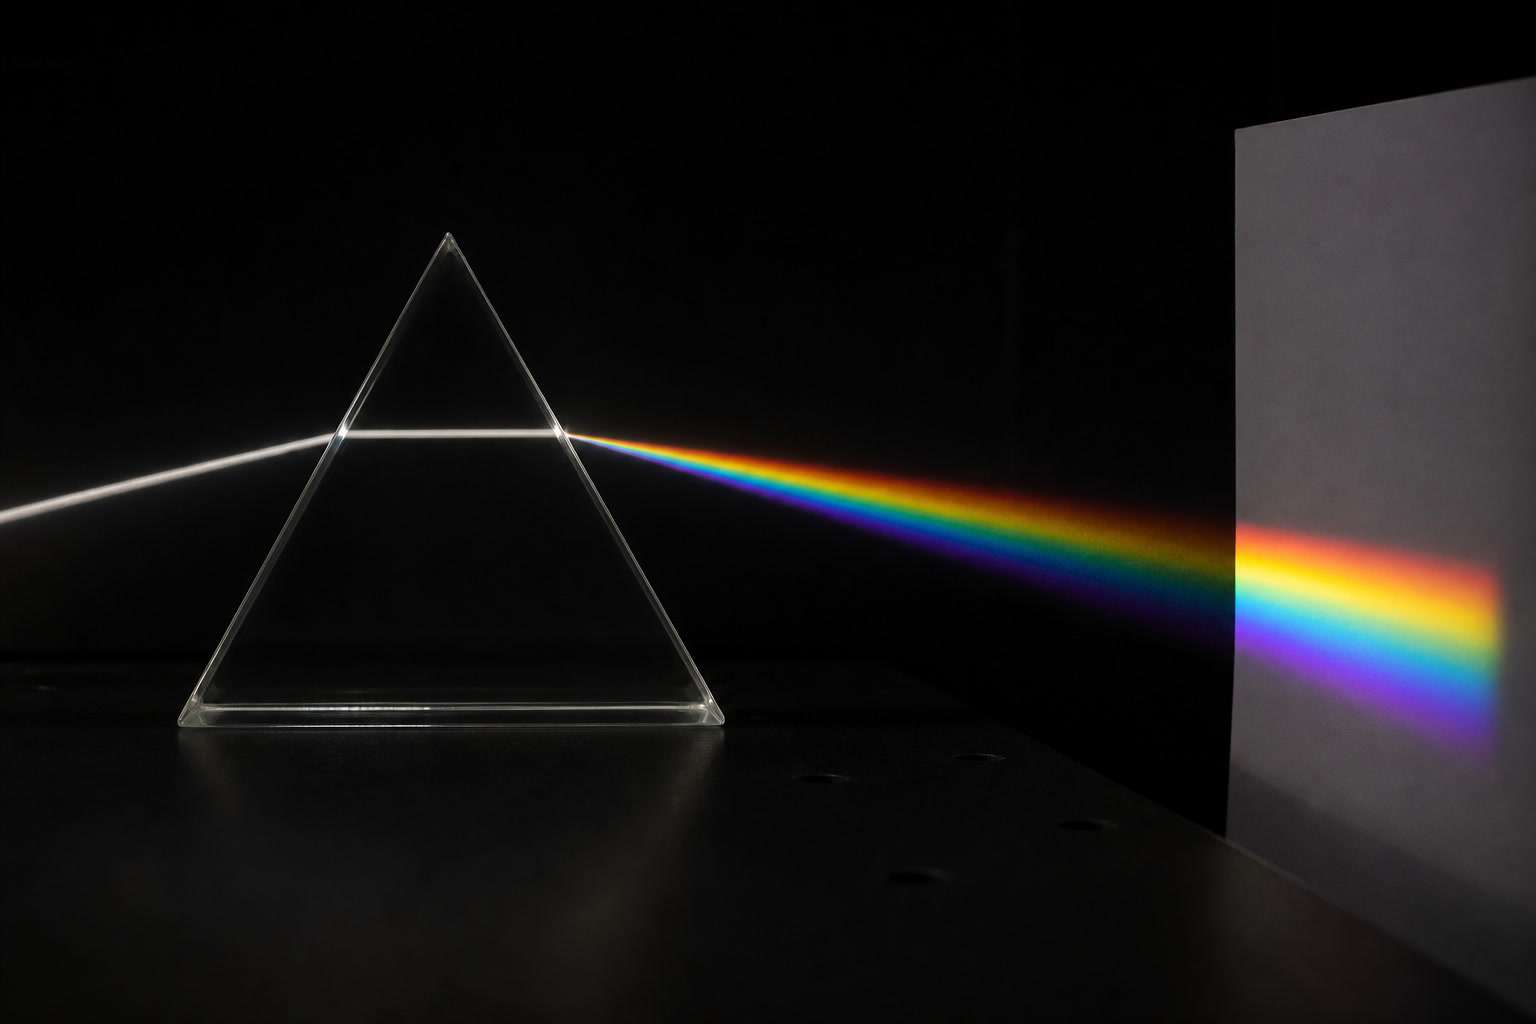
\includegraphics[width=0.55\linewidth]{images/book1/ai/g8-colors-prism.jpg}

{\small 白光经棱镜分解：它原本就含有的各种颜色散开，红色偏折最小，紫色偏折最大。}
\end{omfigure}

\section{苹果为什么是红色的}

\begin{proposition}[物体的颜色]\label{prop:g8:colors-spectra:objectcolor}
不透明物体的颜色是靠“减法”形成的。受到光照时，
物体会\emph{吸收}混合光中的一部分，
并将其余部分漫射出去——漫射出的剩余部分
便是进入眼睛、决定颜色的那一部分。红苹果
几乎吸收了白光中的全部颜色，主要反射出
红色。白纸几乎把所有颜色都反射回来；黑外套
几乎什么也不反射——全部吸收（并因此升温，
夏天的深色汽车便是明证）。颜色并非
\emph{存在于}果皮之中，而是果皮对
所受光照的一种回应。
\end{proposition}

\begin{example}[体育馆实验]\label{ex:g8:colors-spectra:gym}
现在来看灯光偏蓝的体育馆。红苹果的果皮一向如此：
吸收除红色以外的一切颜色，并随时准备反射红色——
但蓝色泛光灯\emph{不含}红光，
无红可反射。既无漫射，也无接收，苹果便显出
黑色。同一灯光下的白纸，只反射它所接收到的
光，于是看起来是蓝色的。舞台上有一条规律：物体只能
反射光所带来的颜色——换了光，
整个大厅里每件“戏服”都会随之改变。
\end{example}

\begin{omfigure}
\begin{tikzpicture}[scale=0.85]
  \fill[omExo, opacity=0.15] (0,0) rectangle (5.2,3.2);
  \draw[-Stealth, very thick] (0.4,2.5) -- (1.7,1.9);
  \node[above, font=\small] at (1.0,2.6) {白光};
  \draw[thick, fill=red!80] (2.4,1.4) circle (0.5);
  \draw[-Stealth, red, very thick] (3.0,1.7) -- (4.4,2.3);
  \node[right, font=\footnotesize, red] at (3.6,2.55)
    {反射出红光};
  \node[below, font=\small] at (2.6,0.3) {呈红色};
  \begin{scope}[xshift=6.4cm]
    \fill[blue!20] (0,0) rectangle (5.2,3.2);
    \draw[-Stealth, very thick, blue] (0.4,2.5) -- (1.7,1.9);
    \node[above, font=\small, blue] at (1.0,2.6) {蓝光};
    \draw[thick, fill=black!85] (2.4,1.4) circle (0.5);
    \node[right, font=\footnotesize] at (3.1,1.9)
      {无光可反射};
    \node[below, font=\small] at (2.6,0.3) {呈黑色};
  \end{scope}
\end{tikzpicture}

{\small 一个苹果，两种光。果皮总是只反射红光
--- 而在蓝光下，已无红光可供反射。}
\end{omfigure}

\begin{method}[任意光照下颜色的预测]\label{met:g8:colors-spectra:predict}
\begin{enumerate}
  \item 列出光所带来的颜色（白光：全部；
        有色灯：主要是其本身的颜色）；
  \item 列出物体在白光下反射的颜色 --- 即其
        日光下的颜色即为其命名；
  \item 取两列表的交集：物体漫射
        两者中共同出现的颜色；
  \item 交集为空：物体呈黑色。
\end{enumerate}
红光下的蓝色帽子：仅反射蓝光，却只提供红光
--- 交集为空：黑色帽子。白光下，全部光照
与蓝色反射相遇 --- 蓝色帽子。
\end{method}

\section{由光构成颜色}

\begin{example}[三盏灯合成万色]\label{ex:g8:colors-spectra:additive}
\emph{光}的混合是相加的。将三盏泛光灯重叠照射 --- 红、
绿、蓝：红与绿合成黄色；绿与
蓝合成青色；蓝与红合成品红；三者
合成白色。由仅仅三种恰当选取的基色出发，光的混合
几乎可以合成人眼能辨别的每一种颜色 --- 这正是
三正是每块发光屏幕的神奇数字。
\end{example}

\begin{example}[口袋里的屏幕]\label{ex:g8:colors-spectra:screen}
用强放大镜观察手机或电视屏幕上的一块白色区域：
看不到任何白色，只有细小的红、绿、
蓝色条纹，全都在发光。屏幕显示的每一种颜色，
都是这三盏灯按一定比例配出的；每一处“白色”，
即是三色全力发光，经
眼睛在一定距离外混合。颜料盒则相反 --- 颜料
吸收光线，混合颜料是减去光而非加上光
--- 这正是混合所有颜料得到浑浊的暗色，而
混合所有光则得到白色；画家的完整故事
属于美术课和化学课。
\end{example}

\begin{remark}[日落，全数兑现]\label{rem:g8:colors-spectra:sunset}
去年的日落之约，如今兑现。空气漫射阳光
--- 但并非一视同仁：混合光中的蓝色一端
比红色容易得多地被散射。白天背离
太阳望去，你所见的是被偷来的那份，由
整个天空转送而来：蓝色。日落时，直射光束
穿过空气的掠射路径最长，蓝色几乎
被偷尽 --- 而抵达你眼睛的幸存者是
红橙色的余光，粉色云朵
接住了晚些时的散射光。蓝天与红色日落是同一次偷窃，从
账本的两面看去。
\end{remark}

\section{练习}

\begin{exercise}[$\star$]\label{exo:g8:colors-spectra:1}
什么是光谱？什么是色散？哪种颜色在棱镜中
偏折最小，哪种偏折最大？
\end{exercise}

\begin{exercise}[$\star$]\label{exo:g8:colors-spectra:2}
为什么观看彩虹的人必须背对太阳站立？
什么起着棱镜的作用？
\end{exercise}

\begin{exercise}[$\star$]\label{exo:g8:colors-spectra:3}
给出两个演示实验，说明白光是复色光 ---
一个将其分开，一个再将其合起来。
\end{exercise}

\begin{exercise}[$\star$]\label{exo:g8:colors-spectra:4}
用减色的语言解释：为什么草是绿色的？为什么白纸
是白色的，黑板是黑色的？
\end{exercise}

\begin{exercise}[$\star$]\label{exo:g8:colors-spectra:5}
用上述方法预测：黄色围巾在白光下；
在蓝光下。
\end{exercise}

\begin{exercise}[$\star$]\label{exo:g8:colors-spectra:6}
为什么红苹果在蓝色体育馆中呈黑色 ---
而旁边的白色手帕却呈蓝色？
\end{exercise}

\begin{exercise}[$\star$]\label{exo:g8:colors-spectra:7}
说出光混合的三种基色，以及
两两重叠的结果 --- 以及三色同时叠加的结果。
\end{exercise}

\begin{exercise}[$\star$]\label{exo:g8:colors-spectra:8}
放大镜能在屏幕的“白色”中看到什么？混合
发生在何处？
\end{exercise}

\begin{exercise}[$\star\star$]\label{exo:g8:colors-spectra:9}
为什么混合所有\emph{光}得到白色，而混合
所有\emph{颜料}却得到浑浊的暗色？对
账本的每个方向各用一句话作答。
\end{exercise}

\begin{exercise}[$\star\star$]\label{exo:g8:colors-spectra:10}
完成日落的账本：空气优先偷走什么，
谁接收这些被偷之物，以何种身份接收，以及什么
能走过最长的掠射路径 --- 以及为何去年的\emph{月食中的月球}
恰好靠这束幸存的光而发亮。
\end{exercise}

\begin{exercise}[$\star\star$]\label{exo:g8:colors-spectra:11}
某商店的试衣间由暖红色的灯照明，
灯光“使肤色显得更好看”。一位顾客买下一件
在暖光下看起来是深暖棕色的夹克，
但在日光下却显得暗淡发绿。请用预测方法
还原这一欺骗过程。
\end{exercise}

\begin{exercise}[$\star\star\star$]\label{exo:g8:colors-spectra:12}
舞台设计：设计师需要一幅横幅，字迹明亮、易读，
在白色观众厅灯光下印于黑色底上。但在结局的深红色
灯光下，整幅横幅——字迹与底色一并——须
均匀地呈黑色而隐没。请从白、红、绿、蓝、黑中
选出字色与底色，
逐一用减色规则论证每项选择，
并说明为何\emph{白色}字迹——这个看似诱人的选择——
会背叛结局。
\end{exercise}

\section{问题：光之剧场}

\begin{problem}[{周末问题——彩色泛光灯下的彩排；
服装、滤光片与一场被破坏的场景；
灯光设计师的考试}]\label{pb:g8:colors-spectra:1}
彩排：三盏泛光灯（红、绿、蓝）配有
调光器、一排服装，以及一份暗藏玄机的剧本。
你掌握着灯光方案。

\medskip\noindent\textbf{第一部分——热身练习。}
\begin{enumerate}
  \item 三盏泛光灯全亮：舞台上是什么光，
        为什么？
  \item 红灯与绿灯全亮、蓝灯熄灭：说出舞台
        的光色。
  \item 在上述红绿混合光下，预测以下物体的样子：白色
        衬衫、蓝色腰带与黄色长袍。
  \item 仅在蓝光下，白色的天幕背景
        ——并说明为何背景幕布总是用白布。
\end{enumerate}

\medskip\noindent\textbf{第二部分——服装会诊。}
\begin{enumerate}[resume]
  \item 反派的外套在第一幕（红光下）须看起来为黑色，
        在第二幕（白光下）却须呈浓郁的绿色。
        日光下呈何种颜色的外套才合适？为什么？
  \item 幽灵的长袍须在
        \emph{每一种}灯光下都看起来为白色。应选何色长袍，
        它在单独每一盏泛光灯下实际会呈现什么颜色？
  \item 一位演员的红色围巾须“隐去”——
        在某一时刻与黑色幕布无从分辨——
        哪些泛光灯可为此戏法而亮，理由何在？
        加入红灯的那一刻，戏法为何失败？
  \item 节目单上的金色字样在正午看上去十分华丽，
        但在偏蓝的晚间预设灯光下却显得浑浊。
        请解释原因，并将金色视为一种暖黄色。
\end{enumerate}

\medskip\noindent\textbf{第三部分——破坏事件。}
开场：布景上的彩虹拱门（涂有条纹：红、
橙、黄、绿、蓝、紫），置于全白光之下。
\begin{enumerate}[resume]
  \item 一名恶作剧者把白光预设换成纯红光。
        逐条条纹来看，观众现在看到什么？
  \item 导演即兴决定，要求同时开启红灯\emph{和}
        蓝灯。哪些条纹会重新显现，
        这种偏品红的灯光对绿色条纹会产生什么影响？
  \item 舞台监督问：为何不能只用
        一盏极亮的单绿灯把拱门“照回正常”？
        请回答：哪一种光能同时显出
        全部六条条纹？
  \item 写出设计师的考卷答案：光之剧场的两条
        定律——一条关于光混合后的表现，
        另一条关于物体如何处置所受之光，
        每条各用一句话表述。
\end{enumerate}
\end{problem}
